%%%%%%%%%%%%%%%%%%%%%%%%%%%%%%%%%%%%%%%%%%%%%%%%%%%%%%%%%%%%%%%%%%%%
%% I, the copyright holder of this work, release this work into the
%% public domain. This applies worldwide. In some countries this may
%% not be legally possible; if so: I grant anyone the right to use
%% this work for any purpose, without any conditions, unless such
%% conditions are required by law.
%%%%%%%%%%%%%%%%%%%%%%%%%%%%%%%%%%%%%%%%%%%%%%%%%%%%%%%%%%%%%%%%%%%%

\documentclass[
  digital,     %% The `digital` option enables the default options for the
               %% digital version of a document. Replace with `printed`
               %% to enable the default options for the printed version
               %% of a document.
%%  color,       %% Uncomment these lines (by removing the %% at the
%%               %% beginning) to use color in the printed version of your
%%               %% document
  oneside,     %% The `oneside` option enables one-sided typesetting,
               %% which is preferred if you are only going to submit a
               %% digital version of your thesis. Replace with `twoside`
               %% for double-sided typesetting if you are planning to
               %% also print your thesis. For double-sided typesetting,
               %% use at least 120 g/m² paper to prevent show-through.
  nosansbold,  %% The `nosansbold` option prevents the use of the
               %% sans-serif type face for bold text. Replace with
               %% `sansbold` to use sans-serif type face for bold text.
  nocolorbold, %% The `nocolorbold` option disables the usage of the
               %% blue color for bold text, instead using black. Replace
               %% with `colorbold` to use blue for bold text.
  lof,         %% The `lof` option prints the List of Figures. Replace
               %% with `nolof` to hide the List of Figures.
  nolot,         %% The `lot` option prints the List of Tables. Replace
               %% with `nolot` to hide the List of Tables.
]{fithesis4}
%% The following section sets up the locales used in the thesis.
\usepackage[resetfonts]{cmap} %% We need to load the T2A font encoding
\usepackage[T1,T2A]{fontenc}  %% to use the Cyrillic fonts with Russian texts.
\usepackage[
  main=slovak, %% By using `czech` or `slovak` as the main locale
                %% instead of `english`, you can typeset the thesis
                %% in either Czech or Slovak, respectively.
  english, german, czech, slovak %% The additional keys allow
]{babel}        %% foreign texts to be typeset as follows:
%%
%%   \begin{otherlanguage}{german}  ... \end{otherlanguage}
%%   \begin{otherlanguage}{czech}   ... \end{otherlanguage}
%%   \begin{otherlanguage}{slovak}  ... \end{otherlanguage}
%%
%%
%% The following section sets up the metadata of the thesis.
\thesissetup{
    date        = \the\year/\the\month/\the\day,
    university  = mu,
    faculty     = fi,
    type        = bc,
    department  = ,
    author      = Adam Renčo,
    gender      = m,
    advisor     = {doc. Ing. Michal Brandejs, CSc.},
    title       = {Potvrdenie o absolvovaní školenia s jednoduchým elektronickým podpisom},
    TeXtitle    = {Potvrdenie o absolvovaní školenia s jednoduchým elektronickým podpisom},
    keywords    = {elektronický podpis, dokumentácia školení, bezpečnosť a ochrana zdravia pri práci, BOZP, požiarna ochrana, PO, elektronické školenie, informačný systém},
    TeXkeywords = {elektronický podpis, dokumentácia školení, bezpečnosť a ochrana zdravia pri práci, BOZP, požiarna ochrana, PO, elektronické školenie, informačný systém
},
    abstract    = {%
Práca sa zaoberá implementáciou jednoduchého elektronického podpisu pre dokumentáciu školení bezpečnosti a ochrany zdravia pri práci a požiarnej ochrany v Informačnom systéme Masarykovej univerzity (IS MU). Riešenie umožňuje digitálne podpisovanie potvrdení o absolvovaní školení priamo v aplikácii Bozp, pričom je zabezpečený súlad so zákonnými požiadavkami na dokumentáciu školení a elektronické podpisy. Prevod dokumentácie do digitálnej formy znižuje administratívnu záťaž pre absolventov aj správcov školení a zefektívňuje správu dokumentácie v IS MU.
    },
    thanks      = {%
Ďakujem docentovi Michalovi Brandejsovi za odborné vedenie mojej bakalárskej práce. Rovnako ďakujem všetkým svojim kolegom za kvalitnú spoluprácu pri úpravách systému a za všetky ich užitočné rady. Poďakovanie by som chcel venovať aj všetkým kamarátom, ktorý ma počas práce podporovali.
    },
    bib         = example.bib,
    %% Remove the following line to use the JVS 2018 faculty logo.
    facultyLogo = fithesis-fi,
}
\usepackage{makeidx}      %% The `makeidx` package contains
\makeindex                %% helper commands for index typesetting.
%% These additional packages are used within the document:
\usepackage{paralist} %% Compact list environments
\usepackage{amsmath}  %% Mathematics
\usepackage{amsthm}
\usepackage{amsfonts}
\usepackage{url}      %% Hyperlinks
\usepackage{markdown} %% Lightweight markup
\usepackage{listings} %% Source code highlighting
\lstset{
  basicstyle      = \ttfamily,
  identifierstyle = \color{black},
  keywordstyle    = \color{blue},
  keywordstyle    = {[2]\color{cyan}},
  keywordstyle    = {[3]\color{olive}},
  stringstyle     = \color{teal},
  commentstyle    = \itshape\color{magenta},
  breaklines      = true,
}
\usepackage{floatrow} %% Putting captions above tables
\floatsetup[table]{capposition=top}
\usepackage[babel]{csquotes} %% Context-sensitive quotation marks
\thesisload
\DeclareDelimFormat{multicitedelim}{\addsemicolon\space}
\DefineBibliographyStrings{slovak}{urlfrom = {dostupné z}}
\begin{document}
%% The \chapter* command can be used to produce unnumbered chapters:
\chapter*{Úvod}
\label{chap:intro}
%% Unlike \chapter, \chapter* does not update the headings and does not
%% enter the chapter to the table of contents. I we want correct
%% headings and a table of contents entry, we must add them manually:
\markright{\textsc{Introduction}}
\addcontentsline{toc}{chapter}{Úvod}
Jednou z dôležitých požiadaviek na prevádzku školení bezpečnosti a ochrany zdravia pri práci (ďalej len BOZP) a požiarnej ochrany (ďalej len PO) je udržiavanie dokumentácie o ich absolvovaní frekventantmi.

Z právnych dôvodov musí byť preukázateľné, že bol daný frekventant korektne zaškolený vo všetkých preňho relevantných smeroch. Aby bola takáto dokumentácia právne nevyvrátiteľná, musí byť schválená ako absolventom školenia, tak aj jeho školiteľom. Informačný systém Masarykovej univerzity (IS MU) používa na tento účel fyzický podpis oboch entít.

Cieľom tejto práce je previezť proces schvaľovania dokumentácie o absolvovaní školení na Masarykovej univerzite (MU) do online formy. Za týmto účelom je nevyhnutná implementácia potvrdení s jednoduchým elektronickým podpisom. Súčasťou práce je aj následný prevod spisov tejto dokumentácie do elektronickej formy. Tieto zmeny uľahčia prácu všetkým zúčastneným stranám prevádzky školení.

Najprv sme preštudovali právne požiadavky na školenia BOZP a PO v kapitole~\hyperref[kap-1]{1} a spôsob prevádzky týchto školení v IS MU v kapitole~\hyperref[kap-2]{2}. Následne sme v kapitole~\hyperref[kap-3]{3} bližšie preskúmali spôsob dokumentácie školení v IS MU a ich nedostatky. Kapitola~\hyperref[kap-4]{4} obsahuje dôležité teoretické základy elektronických podpisov a pečatí. V kapitole~\hyperref[kap-5]{5} sú uvedené relevantné informácie o sade aplikácií pod názvom Úradovňa. Kapitola~\hyperref[kap-6]{6} sa zaoberá možnými riešeniami problémov dokumentácie spomínaných v kapitole~\hyperref[kap-3]{3}. Nakoniec je v kapitole~\hyperref[kap-7]{7} popísaný proces implementácie potvrdení s jednoduchým elektronickým podpisom do systému IS MU.

Výsledné úpravy systému umožňujú frekventantom potvrdiť absolvovanie školenia priamo v IS MU v aplikácii Bozp a zaručujú schválenie školiteľa, ktorým je po týchto úpravách IS MU. Nové potvrdenia o absolvovaní školenia podpísané elektronicky spĺňajú všetky požiadavky na spravovanie dokumentácie BOZP a PO.


\chapter{Školenia BOZP a PO}
\label{kap-1}
V tejto práci sú použité pojmy označujúce osoby, ktoré majú spojenie so školeniami BOZP a PO. Kvôli prehľadnosti ich v tejto kapitole definujeme:

~

    \textbf{Frekventant} je pojem označujúci osobu, ktorá má povinnosť splniť školenie~\cite[9]{kandova2019}.\\
    
    \textbf{Školiteľ} predstavuje entitu (osobu alebo systém), ktorá frekventanta preškoľuje.\\
    
    \textbf{Absolvent} školenia je frekventant, ktorý splnil dané školenie.\\

    \textbf{Správca dokumentácie} je osoba poverená uchovávaním dokumentácie o danom školení.
~
\\\\
Náplň tejto práce je priamo spojená s témou školení BOZP a PO. Z tohto dôvodu je nevyhnutné zhrnúť pár základných informácií na túto tému, ktoré sú dôležité pre porozumenie problémov riešených v nasledujúcich kapitolách.

Zákonník práce Českej republiky nariaďuje zamestnávateľom poskytovať zamestnancom školenia BOZP~\cite[§~103~odst.~3]{cesko_zakonik_prace}, PO~\cite[§~349~odst.~1]{cesko_zakonik_prace} a školenie prvej pomoci~\cite[§~102~odst.~6]{cesko_zakonik_prace}. Zámerom týchto školení je informovanie zamestnancov o možných rizikách, na ktoré môžu pri práci naraziť, a naučenie základných zručností potrebných pre minimalizovanie úrazov a škôd spôsobených v prípade stretu s rizikovou situáciou.

Zákonník ďalej nariaďuje, aby boli frekventanti periodicky preškoľovaní. Frekvenciu si zamestnávateľ stanovuje sám, ale zákon nariaďuje minimum dvoch rokov pre nevedúcich zamestnancov a troch rokov pre vedúcich zamestnancov.~\cite[~§103~odst.~3]{cesko_zakonik_prace}

\section{Variabilita školení}
Presný obsah školení nie je zákonom definovaný. Definované sú iba záchytné body, ktoré sú v školení nevyhnutné. Príkladom je nariadenie, aby školenie PO zahŕňalo požiarny poriadok, požiarne poplachové smernice, prípadne evakuačný plán a ďalšiu dokumentáciu obsahujúcu stanovenie podmienok PO daného pracoviska~\cite[~§23~odst.~1~c)]{cesko_vyhlaska_poziarna_prevence}. Presný obsah tejto dokumentácie je ale v každom školení upravený tak, aby bol relevantný vzhľadom na pracovisko, na ktorom sa školenie prevádzkuje.

K väčšiemu počtu variánt školení prispieva aj fakt, že školenia PO musia byť špecificky upravené pre vedúcich zamestnancov a pre ostatných zamestnancov~\cite[~§16~odst.~2]{cesko_zakon_pozarni_ochrana}. Častokrát tak vznikajú dve verzie k školeniam viazaným na rovnaké pracovisko a pracovnú náplň.

Varianty školení môžu byť označené svojim číslom osnovy. Toto číslo zamestnávateľom obvykle dodáva odborný špecialista BOZP. Pomocou čísla osnovy je následne možné určiť, akým obsahom bol frekventant preškolený. Z tohto dôvodu sa označenie pridáva do dokumentácie o absolvovanom školení, ktorý frekventant a školiteľ podpisujú.

\section{Dokumentácia školení}
Zamestnávateľ je od zákona povinný udržiavať dokumentáciu o tom, že frekventanti absolvovali školenia BOZP a PO~\cites[§~103~odst.~3]{cesko_zakonik_prace}[§~27]{cesko_vyhlaska_poziarna_prevence}.

Táto dokumentácia je následne používaná v právnych procesoch v prípade úrazu alebo škody na pracovisku. Z tohto dôvodu je dôležité, aby bola dokumentácia školení dobre uchovávaná a aby obsahovala všetky relevantné informácie. Zákon presné znenie dokumentácie síce nešpecifikuje, no je odporúčané, aby obsahovali aspoň identifikačné údaje absolventa a školiteľa, informácie o absolvovanom školení a dátum absolvovania~\cite{prevent_bozp}.

\chapter{Školenia v IS MU}
\label{kap-2}
Práca je zameraná na úpravy systému školení v IS MU, preto v nasledujúcej kapitole skrátene popíšeme, ako sú tieto školenia momentálne prevádzkované. 

\section{Aplikácia Bozp}
Frekventanti sa k absolvovaniu školenia dostanú pomocou aplikácie Bozp\footnote{\url{https://is.muni.cz/auth/bozp/}}. V aplikácii Bozp sú školenia tvorené elektronickými kurzami, ktoré môžu obsahovať jednu alebo viac z nasledujúcich častí:
\begin{enumerate}
    \item \textbf{Prezentácia} – obsahuje hlavný výklad a vizuálne materiály.
    \item \textbf{Súbory na stiahnutie} – textové dokumenty, ktoré si účastníci musia stiahnuť a prečítať.
    \item \textbf{Otázky} – test, ktorý musia účastníci správne zodpovedať na overenie porozumenia školenia.~\cite[19]{kandova2019}
\end{enumerate}

\noindent
Hlavný vývojový jazyk IS MU je Perl. Dáta sa ukladajú v databáze Oracle a webové skripty spravuje server Apache. Funkcionalita aplikácie Bozp je obsiahnutá v Perlových moduloch a podporných súboroch v jazykoch Javascript a CSS.

Hlavné moduly pre chod aplikácie sú štyri a každý z nich má svoj špecifický účel:

\begin{itemize}
    \item \textbf{Generický modul} – obsahuje základnú funkcionalitu potrebnú vo všetkých moduloch.
    \item \textbf{Modul pre kurzy} – skladá sa z funkcií potrebných pre správny chod zobrazovania a absolvovania školení a kurzov.
    \item \textbf{Cron modul} – funkcie v ňom sú spúšťané pravidelne a periodicky napríklad pomocou skriptov\footnote{Jednoduchý program alebo súbor s inštrukciami, ktoré sú vykonávané postupne bez potreby manuálnej kompilácie.} spúšťaných cez noc.
    \item \textbf{Správcovský modul} – obsahuje funkcionalitu správcovských aplikácií školení.
\end{itemize}

\noindent
Aplikácia dokáže školenia prikazovať automaticky. Príkazy zakladá pomocou \textbf{pravidiel}, ktoré definujú správcovia školení.~\cite[15]{kandova2019}

\section{Vysoké množstvo dokumentácie o školeniach}
Vzhľadom na povinnosť zamestnávateľa udržiavať dokumentáciu o školeniach je relevantné zistiť koľko variánt školení systém obsahuje a ako často vzniká zamestnancom príkaz na ich absolvovanie. Zistenia sú následne relevantné pre rozhodnutia o forme a udržateľnosti spisov tejto dokumentácie.

\subsection*{Varianty školení a kurzov}
Školenia obsahujú jednu alebo viac verzií kurzov a frekventant si môže vybrať, ktorý kurz absolvuje. Ak je potrebné školenie realizovať vo viacerých jazykoch, pre každú jazykovú variantu sa vytvorí samostatný kurz. Pre úspešné absolvovanie školenia stačí absolvovať ktorýkoľvek kurz patriaci pod toto školenie.

Varianty celých školení majú obvykle svoje číslo osnovy. V prípade, že číslo osnovy nie je so školením dodané, je dôležité uchovávať skrátený obsah školenia, ktorý osnovu nahradzuje.

IS MU obsahuje v čase písania tejto práce viac ako 100 variant školení BOZP a PO a približne 130 kurzov, ktoré tieto školenia realizujú. Toto vysoké množstvo variánt má za následok zvýšené množstvo variánt dokumentov o absolvovaní týchto školení.

\subsection*{Príkazy na absolvovanie školení}
Podľa smernice rektora MU je pre všetkých zamestnancov MU súčasťou povinných školení okrem zákonne povinných školení BOZP a PO aj školenie prvej pomoci~\cites[sekcia~3.2.1,~bod~3.]{smernice_rektora_bozp}.

Tieto školenia majú obmedzenú platnosť. Preto je potrebné priebežne opakovať ich absolvovanie. Frekvencia opakovania je u školení pre vedúcich zamestnancov stanovená na 3 roky~\cites[sekcia~3.2.4,~bod~b)]{smernice_rektora_bozp}[čl.~4,~odst.~2~bod~c)]{smernice_mu_po}. U nevedúcich zamestnancov je táto frekvencia stanovená na 2 roky~\cites[sekcia~3.2.2,~bod~1.]{smernice_rektora_bozp}[čl.~10,~odst.~2]{smernice_mu_po}.

Príkazov na absolvovanie školení tak vzniká veľké množstvo nie len pri prijatí nových zamestnancov, ale aj kvôli postupnému opakovaniu školení po uplynutí ich platnosti. Každé novo absolvované školenie vyžaduje vznik novej dokumentácii o jeho absolvovaní.

\chapter{Dokumentácia školení v IS MU}
\label{kap-3}
V IS MU sa dokumentácia školení uchováva pomocou \textbf{Záznamov o absolvovaní školení} (ďalej len Záznam). Sú to dokumenty formátu PDF\footnote{\url{https://www.adobe.com/cz/acrobat/about-adobe-pdf.html}} generované aplikáciou Bozp. Záznam je definovaný ako dokument, ktorý potvrdzuje, že školiteľ v určený dátum preškolil frekventanta obsahom školení, na ktoré sa Záznam vzťahuje. Pre plnú platnosť Záznamu je potrebné ho vytlačiť, fyzicky podpísať absolventom aj školiteľom a odovzdať správcovi dokumentácie.

Záznamy obsahujú nasledujúce informácie:

\begin{markdown}
  * Informácie o&nbsp;relevantných absolvovaných školeniach;
  * Dátum absolvovania školenia;
  * Identifikačné údaje absolventa;
  * Identifikačné údaje školiteľa (vedúceho zamestnanca);
  * Priestor na podpis absolventa a&nbsp;školiteľa;
  * Meno osoby, ktorej sa Záznam odovzdáva (správca dokumentácie).
\end{markdown}

\section{Podpis a odovzdávanie Záznamov}
Keďže Záznamy vyžadujú podpis fyzickej osoby ako školiteľa, je potrebné túto osobu určiť. Ak nie je vedením špecifikovaná osoba zodpovedná za školenie zamestnancov, je touto povinnosťou poverený priamy nadriadený frekventanta školenia. Záznam o absolvovaní školenia následne musí táto osoba podpísať, čím potvrdzuje, že školenie skutočne prebehlo. V praxi väčšina školení nemá špecifikovanú zodpovednú osobu, a preto sa ďalej budeme zaoberať najmä touto variantou.

Záznamy o všeobecných školeniach, ako napríklad základné školenie BOZP alebo školenie prvej pomoci, podpisujú nadriadený zamestnanci všetkých \textit{kmeňových pracovísk}\footnote{Kmeňové pracovisko - miesto alebo organizačná jednotka, ku ktorej je pracovník formálne pridelený ako svoje hlavné pracovné miesto.} absolventa. Jedna osoba môže mať kmeňových pracovísk na MU akýkoľvek počet.

Záznamy o špecifických školeniach podpisujú nadriadení zamestnanci na pracoviskách (aj iných, ako kmeňových) absolventa, ktoré dané školenie vyžadujú.

Podpísaný Záznam musí absolvent následne odovzdať správcovi dokumentácie. V mnohých prípadoch túto úlohu plní samotný školiteľ, avšak pri každom preškolení je možné presne určiť osobu zodpovednú za správu dokumentácie.

Môže nastať situácia, že zamestnanec školenie absolvuje a počas jeho platnosti vznikne zamestnancovi nový úväzok na inom pracovisku MU, ktoré toto školenie taktiež požaduje. V tomto prípade vedenie MU požiadalo, aby namiesto opakovaného preškoľovania stačilo Záznam o školení dať podpísať školiteľovi (nadriadenému zamestnancovi) na novom pracovisku. Preto musia byť všetky potrebné informácie na generovanie nového Záznamu s iným menom školiteľa uchovávané po celú dobu platnosti školenia.

\section{Skupiny školení v Záznamoch}
Záznamy vyžadujú veľké množstvo administratívnych úkonov spojených s ich uchovávaním. Preto bola na Záznamy stanovená požiadavka, aby mohli obsahovať viacero školení, čím sa ich počet zníži.

Niektoré školenia ale nemôžu spolu patriť do jedného Záznamu. Separátne musia byť napríklad obecné a špecifické školenia, pretože ich treba odovzdávať na iné pracoviská a iným správcom dokumentácie. Prevádzkový odbor rektorátu MU zároveň požiadal, aby školenie pre vodičov nebolo na rovnakom Zozname ako školenia BOZP a PO. Preto sú školenia rozdelené do takzvaných záznamových skupín, ktoré určujú, či môžu byť dve školenia zahrnuté do rovnakého Záznamu.

\section{Problémy so Záznamami}
Záznamy sú síce z právneho hľadiska plne platné, ale spôsob ich generácie a uchovávania so sebou prináša veľké množstvo komplikácií, ktoré ich robia neefektívnymi.

\subsection*{Fyzická forma}
Jednou z najvýraznejších nevýhod je ich fyzická forma. Aj napriek snahám o zjednodušenie ich správy, ako je napríklad spájanie školení do skupín, vyžadujú od absolventov, školiteľov a správcov dokumentácie mnohé úkony, ktoré moderná digitálna forma dokumentácie výrazne zjednodušuje alebo úplne eliminuje.

Častokrát sa napríklad stáva, že zamestnanci Záznam zabudnú odovzdať, odovzdajú nesprávnej osobe, alebo Záznam vôbec ani nevytlačia. Ak by Záznamy boli držané čisto digitálne, všetky tieto akcie by mohli byť automatizované a zjednodušené. Systém by zároveň vedel ľahšie kontrolovať, ktoré akcie už boli vykonané, a upozorniť relevantnú osobu v prípade, že niečo zostalo nedokončené.

Ďalším príkladom je potreba fyzických spisov. Systém neobsahuje úložisko vytlačených Záznamov, a preto sú Záznamy udržiavané iba vo fyzických spisoch správcami dokumentácie. Táto potreba by taktiež bola digitalizáciou úplne odstránená.

\subsection*{Podpis Záznamu na novom pracovisku}
Ak zamestnanec nastúpi na nové pracovisko, ale niektoré požadované školenie už má absolvované a platné, nie je ním preškolený znova. Namiesto školenia mu nový nadriadený zamestnanec podpíše Záznam o školení ako jeho školiteľ.

Komplikáciu predstavuje fakt, že Záznam z definície tvrdí, že daný školiteľ preškolil frekventanta daným školením v určenom dátume. Ak je na Zázname nové dátum školenia (po vzniku nového úväzku), tak je toto tvrdenie nepravdivé, pretože ku žiadnemu preškoleniu neprišlo. Takisto však nový nadriadený zamestnanec nemôže podpísať Záznam o školení s dátumom, v ktorom zamestnanec školenie reálne absolvoval, pretože v danej dobe ešte nebol nadriadeným tohto zamestnanca.

\subsection*{Dynamická generácia}
Za určitých okolností je nutné Záznam generovať nanovo. Nová generácia je potrebná najmä pri zmenách, ako sú napríklad pridanie školenia rovnakej záznamovej skupiny školení alebo prestup na nové pracovisko. Táto potreba so sebou prináša problémy s udržiavaním histórie dát.

Keďže sa v digitálnej forme Záznamy neuchovávajú, musí byť každý Záznam generovaný nanovo. V prípade, že sa zmení legislatíva alebo iné parametre, ktoré sú súčasťou Záznamov, môže nastať problém so spiatočnou generáciou. Záznam vygenerovaný pre školenie absolvované pred zmenami by totiž nemusel predstavovať korektnú dokumentáciu o jeho absolvovaní.

\section{Zvažované úpravy}
Veľké množstvo problémov Záznamov je úzko späté s ich fyzickou formou. Preto je hlavným zvažovaným riešením pre IS MU prevod tejto dokumentácie do digitálnej formy, v ktorej by mohli byť procesy jej prevádzky zjednodušené a automatizované.


\chapter{Elektronická identifikácia a dôveryhodné služby}
\label{kap-4}
Aby bolo možné dokumentáciu previezť do digitálnej formy, je dôležité, aby boli zachované jej právne účinky. Na tento účel sa v elektronických dokumentoch používajú elektronické podpisy a elektronické pečate, ktoré v tejto kapitole rozoberieme.

Nariadenia Európskej únie (ďalej len EÚ) č. 910/2014 a č. 2024/1183 (citované v ich konsolidovanej verzii) o elektronickej identifikácii a dôveryhodných službách pre elektronické transakcie na vnútornom trhu (ďalej len eIDAS) definujú kľúčové pojmy týkajúce sa elektronických podpisov a elektronických pečatí. V nariadeniach sú tieto pojmy vyložené s cieľom zabezpečiť právnu istotu a interoperabilitu elektronickej identifikácie v rámci členských štátov EÚ~\cite{eidas2024}. Pre správne porozumenie legislatívnych požiadaviek týkajúcich sa elektronických identifikačných prostriedkov je nevyhnutné jasne vymedziť pojmy použité v týchto dokumentoch.

\textbf{Elektronický podpis} je v eIDAS definovaný ako akékoľvek dáta v elektronickej podobe, ktoré sú pripojené k iným dátam v elektronickej podobe, alebo sú s nimi logicky spojené a podpisujúca osoba ich používa k podpísaniu~\cite[čl.~3,~odst.~10]{eidas2024}. Elektronický podpis nesmie byť zamietnutý ako dôkaz a nesmú mu byť odopreté právne účinky čisto z dôvodu, že má elektronickú podobu alebo nespĺňa požiadavky kvalifikovaného elektronického podpisu~\cite[čl.~25,~odst.~1]{eidas2024}.

Pod pojmom \textbf{fyzická osoba} sa rozumie ľudská bytosť, ktorá je právnym subjektom schopným využívať elektronické identifikačné a dôveryhodné služby. \textbf{Podpisujúca osoba} je definovaná ako fyzická osoba, ktorá vytvára elektronický podpis~\cite[čl.~3,~odst.~9]{eidas2024}.

\textbf{Elektronická pečať} sú elektronické dáta priamo alebo logicky pripojené k iným dátam v elektronickej podobe za účelom zachovania ich pôvodu a integrity~\cite[čl.~3,~odst.~25]{eidas2024}.

Pojem \textbf{právnická osoba} označuje akúkoľvek entitu, ako je spoločnosť, združenie alebo organizácia, ktorá má právnu spôsobilosť a je uznávaná právom. \textbf{Pečatiaca osoba} je právnická osoba, ktorá vytvára elektronickú pečať~\cite[čl.~3,~odst.~9]{eidas2024}.

\textbf{Dáta pre vytváranie elektronických podpisov} sú jedinečné dáta, pomocou ktorých podpisujúca osoba vytvára svoje elektronické podpisy~\cite[čl.~3,~odst.~13]{eidas2024}.

\textbf{Prostriedok pre vytváranie elektronických podpisov} je programové vybavenie alebo technické zariadenie, ktoré sa používa pre vytváranie elektronických podpisov\cite[čl.~3,~odst.~22]{eidas2024} .\textbf{Kvalifikovaný prostriedok pre vytváranie elektronických podpisov} je prostriedok pre vytváranie elektronických podpisov, ktorý spĺňa nasledujúce podmienky~\cite[čl.~3,~odst.~23]{eidas2024}:

\begin{itemize}
  \item Zaisťuje dôvernosť dát pre vytváranie elektronických podpisov, ktoré boli použité pri vytváraní elektronického podpisu;
  \item zaisťuje, aby dáta pre vytváranie elektronických podpisov použité pre vytváranie elektronického podpisu mohli byť prakticky použité iba raz;
  \item zaisťuje neodvoditeľnosť dát pre vytváranie elektronických podpisov použitých pre vytváranie elektronického podpisu~a ochranu elektronického podpisu v súčasnosti dostupnými technickými prostriedkami proti falšovaniu;
  \item zaisťuje, že podpisujúca osoba mala možnosť spoľahlivo ochrániť dáta pre vytváranie elektronických podpisov použité pre vytváranie elektronického podpisu pred ich zneužitím inou osobou; a
  \item nemení podpisované dáta~a nebráni tomu, aby tieto dáta boli pred podpísaním predložené podpisujúcej osobe.~\cite[príloha II]{eidas2024}
\end{itemize}

\noindent
Prostriedkom pre vytváranie elektronických podpisov sú napríklad aplikácie umožňujúce tvorenie elektronických podpisov, hardvérové zariadenia obsahujúce dáta pre vytváranie elektronických podpisov alebo biometrické zariadenia používané pre potvrdenie identity podpisujúcej osoby. 

Aby bol elektronický podpis považovaný za \textbf{zaručený elektronický podpis}, musí spĺňať nasledujúce podmienky~\cite[čl.~3,~odst.~11]{eidas2024}:

\begin{itemize}
    \item Je jednoznačne spojený s podpisujúcou osobou;
    \item umožňuje identifikáciu podpisujúcej osoby;
    \item je vytvorený pomocou dát pre vytváranie elektronických podpisov a podpisujúca osoba tieto dáta dokáže s vysokou úrovňou dôvery použiť pod svojou výhradnou kontrolou; a
    \item je pripojený k dátam, ktoré podpisuje, takým spôsobom, aby bolo možné zistiť ich akúkoľvek následnú zmenu.~\cite[čl.~26]{eidas2024}
\end{itemize}

\noindent
\textbf{Dáta pre overovanie platnosti} sú dáta používané k overeniu platnosti elektronického podpisu alebo elektronickej pečate~\cite[čl.~3,~odst.~40]{eidas2024}.

Za \textbf{službu vytvárajúcu dôveru} sa považuje elektronická služba poskytovaná za finančnú odmenu a zabezpečuje rôzne činnosti súvisiace s elektronickými podpismi a ďalšími službami, ktoré sú nevyhnutné na zaručenie dôvery pri elektronických transakciách~\cite[čl.~3,~odst.~16]{eidas2024}. \textbf{Kvalifikovanou službou vytvárajúcou dôveru} je služba vytvárajúca dôveru, ktorá splňuje použiteľné požiadavky v nariadení eIDAS~\cite[čl.~3,~odst.~17]{eidas2024}.

Pojem \textbf{Poskytovateľ služieb vytvárajúcich dôveru} označuje akúkoľvek fyzickú alebo právnickú osobu, ktorá poskytuje službu vytvárajúcu dôveru~\cite[čl.~3,~odst.~19]{eidas2024}. \textbf{Kvalifikovaný poskytovateľ služieb vytvárajúcich dôveru} je poskytovateľ služieb vytvárajúcich dôveru, ktorý poskytuje kvalifikovanú službu vytvárajúcu dôveru a ktorému bol udelený status kvalifikovaného poskytovateľa orgánom dohľadu~\cite[čl.~3,~odst.~20]{eidas2024}.

\textbf{Certifikát per elektronický podpis} je elektronické potvrdenie, ktoré spojuje dáta pre overovanie platnosti podpisu s fyzickou osobou a potvrdzuje minimálne jej meno alebo pseudonym\footnote{Pseudonym - fiktívne meno používané osobou na skrytie svojej pravej identity}~\cite[čl.~3,~odst.~14]{eidas2024}. \textbf{Kvalifikovaným certifikátom pre elektronický podpis} je každý certifikát pre elektronický podpis, ktorý je vydaný kvalifikovaným poskytovateľom služieb vytvárajúcich dôveru a obsahuje všetky informácie požadované v prílohe I nariadenia eIDAS~\cites[čl.~3,~odst.~15]{eidas2024}[príloha I]{eidas2024}.

\textbf{Kvalifikovaný elektronický podpis} je zaručený elektronický podpis, ktorý je vytvorený kvalifikovaným prostriedkom pre vytváranie elektronických podpisov a založený na kvalifikovanom certifikáte pre elektronické podpisy~\cite[čl.~3,~odst.~12]{eidas2024}. Z právneho hľadiska má takto definovaný kvalifikovaný elektronický podpis rovnaké právne účinky ako vlastnoručný podpis dokumentu~\cite[čl.~25,~odst.~2]{eidas2024}.

\textbf{Jednoduchý elektronický podpis} je akýkoľvek elektronický podpis, ktorý nespĺňa podmienky kvalifikovaného elektronického podpisu ani zaručeného elektronického podpisu. Príkladom takéhoto podpisu je napríklad sken vlastnoručného podpisu, pripojenie svojho mena na koniec správy alebo potvrdenie identity pomocou stlačenia tlačidla.

Presnejšie vymedzenia platnosti jednotlivých elektronických podpisov si upravujú členské štáty EÚ vo vlastnej štátnej legislatíve. Pre potreby dokumentácie školení BOZP a PO je v Českej republike možné použiť akýkoľvek druh elektronického podpisu vrátane jednoduchého elektronického podpisu~\cite[§~7]{cesko_el_podpisy}.


\chapter{Úradovňa}
\label{kap-5}
Vzhľadom na zvažovaný prevod dokumentácie školení do digitálnej formy je dôležité popísať sadu aplikácií v IS MU pod názvom Úradovňa\footnote{\url{https://is.muni.cz/auth/uradovna/}}. Úradovňa v sebe zahŕňa kompletnú digitálnu spisovú službu, ktorá eviduje komunikáciu medzi školou a ostatnými subjektami, a evidenciu postupu riešenia daných vecí. Ponúka aj možnosť automatickej kontroly, automatického doplňovania údajov a ich hromadného zadávania.~\cite{uradovna2024}

Úradovňa je primárne určená na ukladanie a správu údajov v elektronickej podobe. K týmto elektronicky evidovaným dátam je možné pripojiť aj dokumenty vo fyzickej podobe vrátane naskenovaných verzií dokumentov.~\cite{uradovna2024}

V Úradovni je základnou jednotkou spis. Táto jednotka analogicky k papierovým spisom obsahuje všetky relevantné informácie o určitej záležitosti. K spisu môžu byť pridané atribúty pre upresnenie osôb a vecí, ktorých sa týka. Každý spis sa skladá z úkonov a patrí do jednej agendy.~\cite{uradovna2024}

Úkony predstavujú údaje držané v danom spise. Takisto môžu obsahovať upresňujúce atribúty.~\cite{uradovna2024} Úkonom môže byť napríklad založenie spisu, vloženie dokumentu, ale aj pre túto prácu relevantnejšie podpísanie dokumentu a zapečatenie dokumentu.

Agendy sú tvorené spismi, ktoré evidujú záležitosti rovnakého charakteru. Nastavenie agendy určuje, aké atribúty majú spisy a úkony, ktoré do nej spadajú. Každá agenda je následne priradená na správu konkrétnemu pracovisku.~\cite{uradovna2024}

Úradovňa takisto ponúka aj nastavenia prístupových práv k udržiavaným dokumentom. Existuje implicitný a explicitný druh práv. Implicitné práva na prístup vznikajú pre osobu, ktorej sa spis týka, a zároveň pre všetky osoby, od ktorých je žiadaný úkon do daného spisu. Explicitné práva sú potrebné pre administratívnu stránku držania dokumentácie. V kontexte dokumentácie školení je najdôležitejším právo j\_spis. Toto právo je viazané na pracovisko a umožňuje čítanie spisov a pridávanie úkonov v jeho agendách~\cite{uradovna2024}.

\chapter{Návrh možností}
\label{kap-6}
Záznamy ako dokumentácia absolvovaných školení so sebou zjavne prinášajú veľké množstvo problémov. Hlavnou motiváciou tejto práce je práve úprava systému tak, aby boli tieto problémy minimalizované alebo úplne odstránené. Za týmto účelom sme preskúmali rôzne možnosti úprav aplikácií v rámci IS MU, ktoré podrobnejšie rozoberieme v tejto kapitole.

Riešenia sú založené na digitalizácii dokumentácie absolvovaných školení. Ako digitálna spisová služba je používaná Úradovňa vysvetlená v kapitole~\hyperref[kap-5]{5}.

Na účel elektronickej identifikácie dokumentácie bol po konzultácii s Právnym odborom MU zvolený jednoduchý elektronický podpis. Podľa zákona je dostačujúci (vysvetlené v kapitole~\hyperref[kap-4]{4}) a pre používateľov je praktickejší, pretože nevyžaduje vlastníctvo špeciálneho certifikátu ani zariadenia. Zaručené a kvalifikované elektronické podpisy sú bezpečnejšie, ale ich získanie je náročnejšie z administratívneho aj technického hľadiska, keďže vyžadujú certifikáciu od kvalifikovaných poskytovateľov dôveryhodných služieb a často aj používanie bezpečnostného hardvéru.

\section{Presun Záznamov do aplikácie Úradovňa}
Pôvodný zámer správy Záznamov bol, že po ich vytlačení budú v papierovej forme podpísané školiteľom aj absolventom a následne naskenované a vložené do digitálneho spisu absolventa. Sken vlastnoručných podpisov spĺňa požiadavky jednoduchého elektronického podpisu. Riešenie by využilo funkcionalitu aplikácie Úradovňa pre spracovávanie papierových dokumentov do spisov. 

Záznamy by bolo potrebné označiť, aby sa dali efektívne skenovať a digitálne skladovať. Skenovanie dokumentov v Úradovni funguje pomocou čiarových kódov~\cite{uradovna2024}, a preto by v aplikácii Bozp bolo potrebné implementovať podporu pre tvorbu čiarových kódov, ktoré by boli rozpoznateľné v oboch aplikáciách. Touto úpravou by vznikli elektronické spisy o školeniach, ktoré sú prehľadnejšie a efektívnejšie ako tie fyzické.

Ostatné problémy Záznamov by táto úprava ale vôbec nevyriešila. Záznamy by stále požadovali vytlačenie do papierovej formy, podpísanie školiteľa aj absolventa a vznikla by potreba Záznam naskenovať miesto odovzdania správcovi dokumentácie. 

Ďalším závažným problémom riešenia je overenie obsahu skenovaného dokumentu. Spisová služba Úradovne dokáže rozoznať čiarový kód a dokument zaradiť k relevantnému spisu. Nemá ale ako overiť, že daný naskenovaný dokument obsahuje presne to, čo o jeho obsahu tvrdí jeho čiarový kód. Do spisov by sa tak mohli dostať nesprávne alebo falošné dokumenty v prípade, že by boli označené čiarovým kódom pre tento spis.

\section{Digitalizovanie Záznamov a podpis v Úradovni}
Následne vznikol návrh Záznamy previezť z fyzickej formy do digitálnej a udržiavať ich v Úradovni. Po absolvovaní školenia by bol Záznam digitálne presunutý do spisu absolventa a v spise elektronicky podpísaný školiteľom a absolventom.

Oproti predošlému návrhu by tak neboli potrebné žiadne administratívne úkony s fyzickými dokumentami. Správcom dokumentácie by sa v Úradovni ľahšie kontrolovalo, či sú Záznamy podpísané oboma osobami. Zároveň by nebolo Záznamy potrebné skenovať, takže by riešenie eliminovalo problém s overovaním obsahu skenovaného dokumentu. Aplikácia Bozp by iba finálny Záznam interne predala do Úradovne.

Takáto úprava ale stále nerieši ostatné problémy Záznamov. V prípade úväzkov na viacerých pracoviskách by vznikali komplikácie s vznikom viacerých Záznamov k jednému školeniu. Muselo by vzniknúť viacero rozdielnych Záznamov pre rovnaké školenia a pre každý Záznam by bolo potrebné založiť separátny spis na konkrétnom pracovisku absolventa. Rovnako pretrvávajú aj problémy určovania školiteľa a správcu dokumentácie pre daný Záznam. Vyriešený nie je ani problém dynamickej generácie Záznamov.

\section{Prechod zo Záznamov na Potvrdenia}
Problémy predošlého riešenia už ale nevznikajú kvôli fyzickej forme Záznamov, ale priamo kvôli ich definícii a spôsobu generácie. Finálnym návrhom, ktorý je použitý v implementačnej časti tejto práce, je prechod pri dokumentácii o absolvovaných školeniach od Záznamov k \textbf{Potvrdeniam o absolvovaní školenia s jednoduchým elektronickým podpisom} (ďalej len Potvrdenie). Potvrdenie je dokument formátu PDF generovaný aplikáciou Bozp. Je definované ako dokument, ktorý potvrdzuje, že daný frekventant absolvoval špecifikované školenie v určitý dátum. Pre jeho nevyvrátiteľnosť je Potvrdenie podpísané jednoduchým podpisom absolventa a zabezpečený kvalifikovanou elektronickou pečaťou IS MU.

\subsection*{Obsah}
Vďaka prevodu tejto dokumentácie do elektronickej formy je možné uvoľniť a v niektorých prípadoch úplne odstrániť požiadavky, ktoré boli stanovené pre Záznamy. 
Frekventanti školenie absolvujú pomocou elektronických kurzov v aplikácii Bozp v IS MU bez dozoru nadriadeného zamestnanca alebo inej poverenej osoby. Preto nie je potrebné ako školiteľa špecifikovať fyzickú osobu. Ako školiteľ v tejto situácii pôsobí samotný IS MU, a preto je dostačujúce, aby bolo Potvrdenie podpísané absolventom.
Digitálna forma dokumentácie uľahčuje procesy podpisu a správy. Vďaka tejto výhode nie je potrebné tvoriť záznamové skupiny školení a zhlukovať dokumentáciu o absolvovaných školeniach do jedného Potvrdenia. Každé Potvrdenie sa vzťahuje práve na jedno školenie jedného absolventa v určitom dátume. Táto zmena znižuje zložitosť generácie dokumentácie a odstraňuje komplikácie, ktoré vznikajú použitím záznamových skupín.

Obsah Potvrdenia tvoria:

\begin{itemize}
  \item Identifikačné údaje absolventa;
  \item informácie o absolvovanom školení a jeho obsah;
  \item dátum absolvovania školenia; a
  \item podpisová doložka s jednoduchým elektronickým podpisom absolventa.
\end{itemize}

\subsection*{Podpis a pečatenie}
Potvrdenia sú navrhnuté so snahou čo najviac digitalizovať túto dokumentáciu. Preto nevyžadujú vlastnoručný fyzický podpis. Namiesto vytlačenia do papierovej formy a následného podpisu má frekventant po úspešnom dokončení základných 3 častí kurzu školenia (časti definované v kapitole~\hyperref[kap-2]{2}) možnosť podpísať Potvrdenie o absolvovaní školenia pomocou stlačenia tlačidla s textom \enquote{Podpísať}. 

Takýto podpis splňuje prvú časť definície elektronického podpisu. Stlačením tlačidla sa vygenerujú dáta, ktoré sú s dokumentom logicky spojené a pochádzajú od podpisujúcej osoby. Na splnenie druhej časti definície je nevyhnutné preukázať, že zámerom vygenerovania týchto dát pomocou stlačenia tlačidla podpisujúcou osobou je podpísať dokument. Táto podmienka je splnená textom nadpisu v aplikácii, ktorý žiada osobu o podpísanie Potvrdenia, a nápisom \enquote{Podpísať} na tlačidle, ktorý špecifikuje, že akcia jeho stlačenia daný dokument podpíše.

Jednoduchý elektronický podpis podľa definície nie je zaručený. Preto nie je garantované, že ho k dokumentu pripojila práve osoba, ku ktorej sa podpis vzťahuje~\cite{navara2021}. Možnosť podpísať Potvrdenie je z toho dôvodu prístupná iba používateľom v autentizovanom režime IS MU. Do tohto režimu sa používateľ dostane iba po prihlásení do systému pomocou prihlasovacieho mena a hesla, ktoré náležia iba majiteľovi účtu. Vďaka histórii činností používateľa držanej v IS MU je potom lepšie preukázateľné, že jednoduchý elektronický podpis naozaj k dokumentu priložil samotný používateľ.

Jednoduchý elektronický podpis takisto nezaručuje integritu podpísaného dokumentu. Za týmto účelom Právny odbor MU požiadal, aby boli Potvrdenia chránené pred manipuláciou po elektronickom podpísaní absolventom. IS MU vlastní kvalifikovanú elektronickú pečať. Po podpise je Potvrdenie touto pečaťou zapečatené. Pomocou kvalifikovanej elektronickej pečate je preukázateľný pôvod dokumentu z IS MU a zachovanie jeho integrity od momentu zapečatenia.

\subsection*{Uchovávanie}
Potvrdenia, ako dokumentáciu o absolvovaných školeniach, má zamestnávateľ povinnosť dlhodobo udržiavať. Záznamy na tento účel používajú fyzické spisy, ktoré spravujú správcovia dokumentácie. Potvrdenia sú ale plne funkčné v digitálnej forme. Na ich správu nie je potrebné ich papierové formy udržiavať vo fyzických spisoch.

Namiesto fyzických spisov sú Potvrdenia držané v digitálnych spisoch Úradovne. Aplikácia Bozp po dokončení kurzu vytvorí Potvrdenie a poskytne ho frekventantovi na podpísanie. V momente, ako frekventant Potvrdenie podpíše, je dokument interne predaný z aplikácie Bozp do Úradovne. Tá spojí dokument s podpisovou doložkou, ktorá obsahuje všetky relevantné informácie o jednoduchom elektronickom podpise absolventa, a pridá k dokumentu formálne náležitosti spisovej služby vrátane čiarového kódu pre jeho identifikáciu. Následne dokument zapečatí kvalifikovanou pečaťou IS MU a v tejto forme udržiava v spise. V spise sú držané všetky úkony, ktoré boli vykonané, a pečať garantuje pôvod a integritu finálneho dokumentu.

Záznamy museli byť odovzdávané na všetky kmeňové pracoviská zamestnanca alebo prípadne na všetky pracoviská zamestnanca požadujúce školenia na danom Zázname. Pri Potvrdeniach vďaka ich digitálnej forme a dostupnosti nie je nutné vytvárať takéto kópie. Namiesto toho je jediný dokument vygenerovaný a uložený v spise Úradovne. Tento spis je spojený s jedným vybraným pracoviskom absolventa. Ostatné pracoviská, ktoré toto Potvrdenie požadujú, dostanú právo na prístup k danému spisu. Týmto spôsobom sú oveľa jednoduchšie vyriešené komplikácie pri vzniku úväzku na inom pracovisku MU, ktoré od zamestnanca požaduje akékoľvek ním už absolvované školenie.

Je ale nevyhnutné, aby boli spisy v Úradovni stále pod kontrolou správcov dokumentácie. Preto je dôležité pre každé pracovisko, ktoré bude takéto spisy udržiavať, vybrať osobu zodpovednú za túto dokumentáciu a prideliť jej práva na požadované administratívne úkony.

\chapter{Implementácia Potvrdení do IS MU}
\label{kap-7}
V tejto kapitole popíšeme najdôležitejšie časti procesu implementácie Potvrdení do IS MU pomocou úprav v aplikácii Bozp a jej spojením s Úradovňou.

Aplikácia Bozp je v aktívnom prevádzkovom režime. Preto je pri vykonávaní zmien dôležité nenarušiť doterajšiu funkcionalitu, ktorú aplikácia poskytuje, a neznehodnotiť existujúce dáta s ňou spojené.

\section{Generácia Potvrdení}
Finálne Potvrdenia sú dokument formátu PDF. Kvôli ich zložitým formátovacím a vizuálnym prvkom je ale výhodnejšie proces ich generácie rozdeliť na dve fázy.

V prvej fáze sa vytvorí súbor vo formáte \TeX\footnote{\url{https://petr.olsak.net/ftp/olsak/bulletin/tb115olsak-bib.pdf}}. Tento súbor je generovaný pomocou šablóny potvrdenia v jazyku \TeX. Následne sa z databázy načítajú dôležité informácie o absolventovi a jeho absolvovanom školení. Špecifické dáta sú vložené na vyhradené miesta v šablóne potvrdenia.

V druhej fáze sa zo súboru vo formáte \TeX{} pomocou \TeX-ového servera vytvorí PDF súbor, ktorý je pre používateľov vizuálne prehľadnejší a ľahšie zrozumiteľný. Tento PDF súbor predstavuje finálnu nepodpísanú verziu Potvrdenia.

Obsah školenia v Potvrdení môže byť špecifikovaný stručne alebo celkovo. Môže nastať aj prípad, že sú špecifikované oba druhy obsahu. V takom prípade sú do výsledného Potvrdenia vložené oba obsahy. 

Potvrdenia poskytujú možnosť generácie obsahu v kombinácii češtiny a angličtiny, aby ich mohli využívať aj zamestnanci, ktorý český jazyk nepoužívajú.V prípade žiadosti Potvrdenia v oboch jazykoch sú vyhotovené obe jazykové varianty a pripojené za sebou do jedného dokumentu.

\section{Úprava školení v aplikácii Bozp}
Funkcionalita poskytovania školení a zobrazovania kurzov je obsiahnutá najmä v module pre kurzy. Dôležité je ale upraviť aj generický modul, ktorého funkcie sú v module pre kurzy často používané.

Po vstupe do akéhokoľvek vybraného kurzu zobrazuje aplikácia Bozp prehľad obsahu vybraného kurzu. K 3 základným častiam popísaným v kapitole~\hyperref[kap-2]{2} je pridaná časť, v ktorej je od frekventanta žiadaný podpis Potvrdenia (pozri obr.~\ref{obr1}).

\begin{figure}
  \begin{center}
    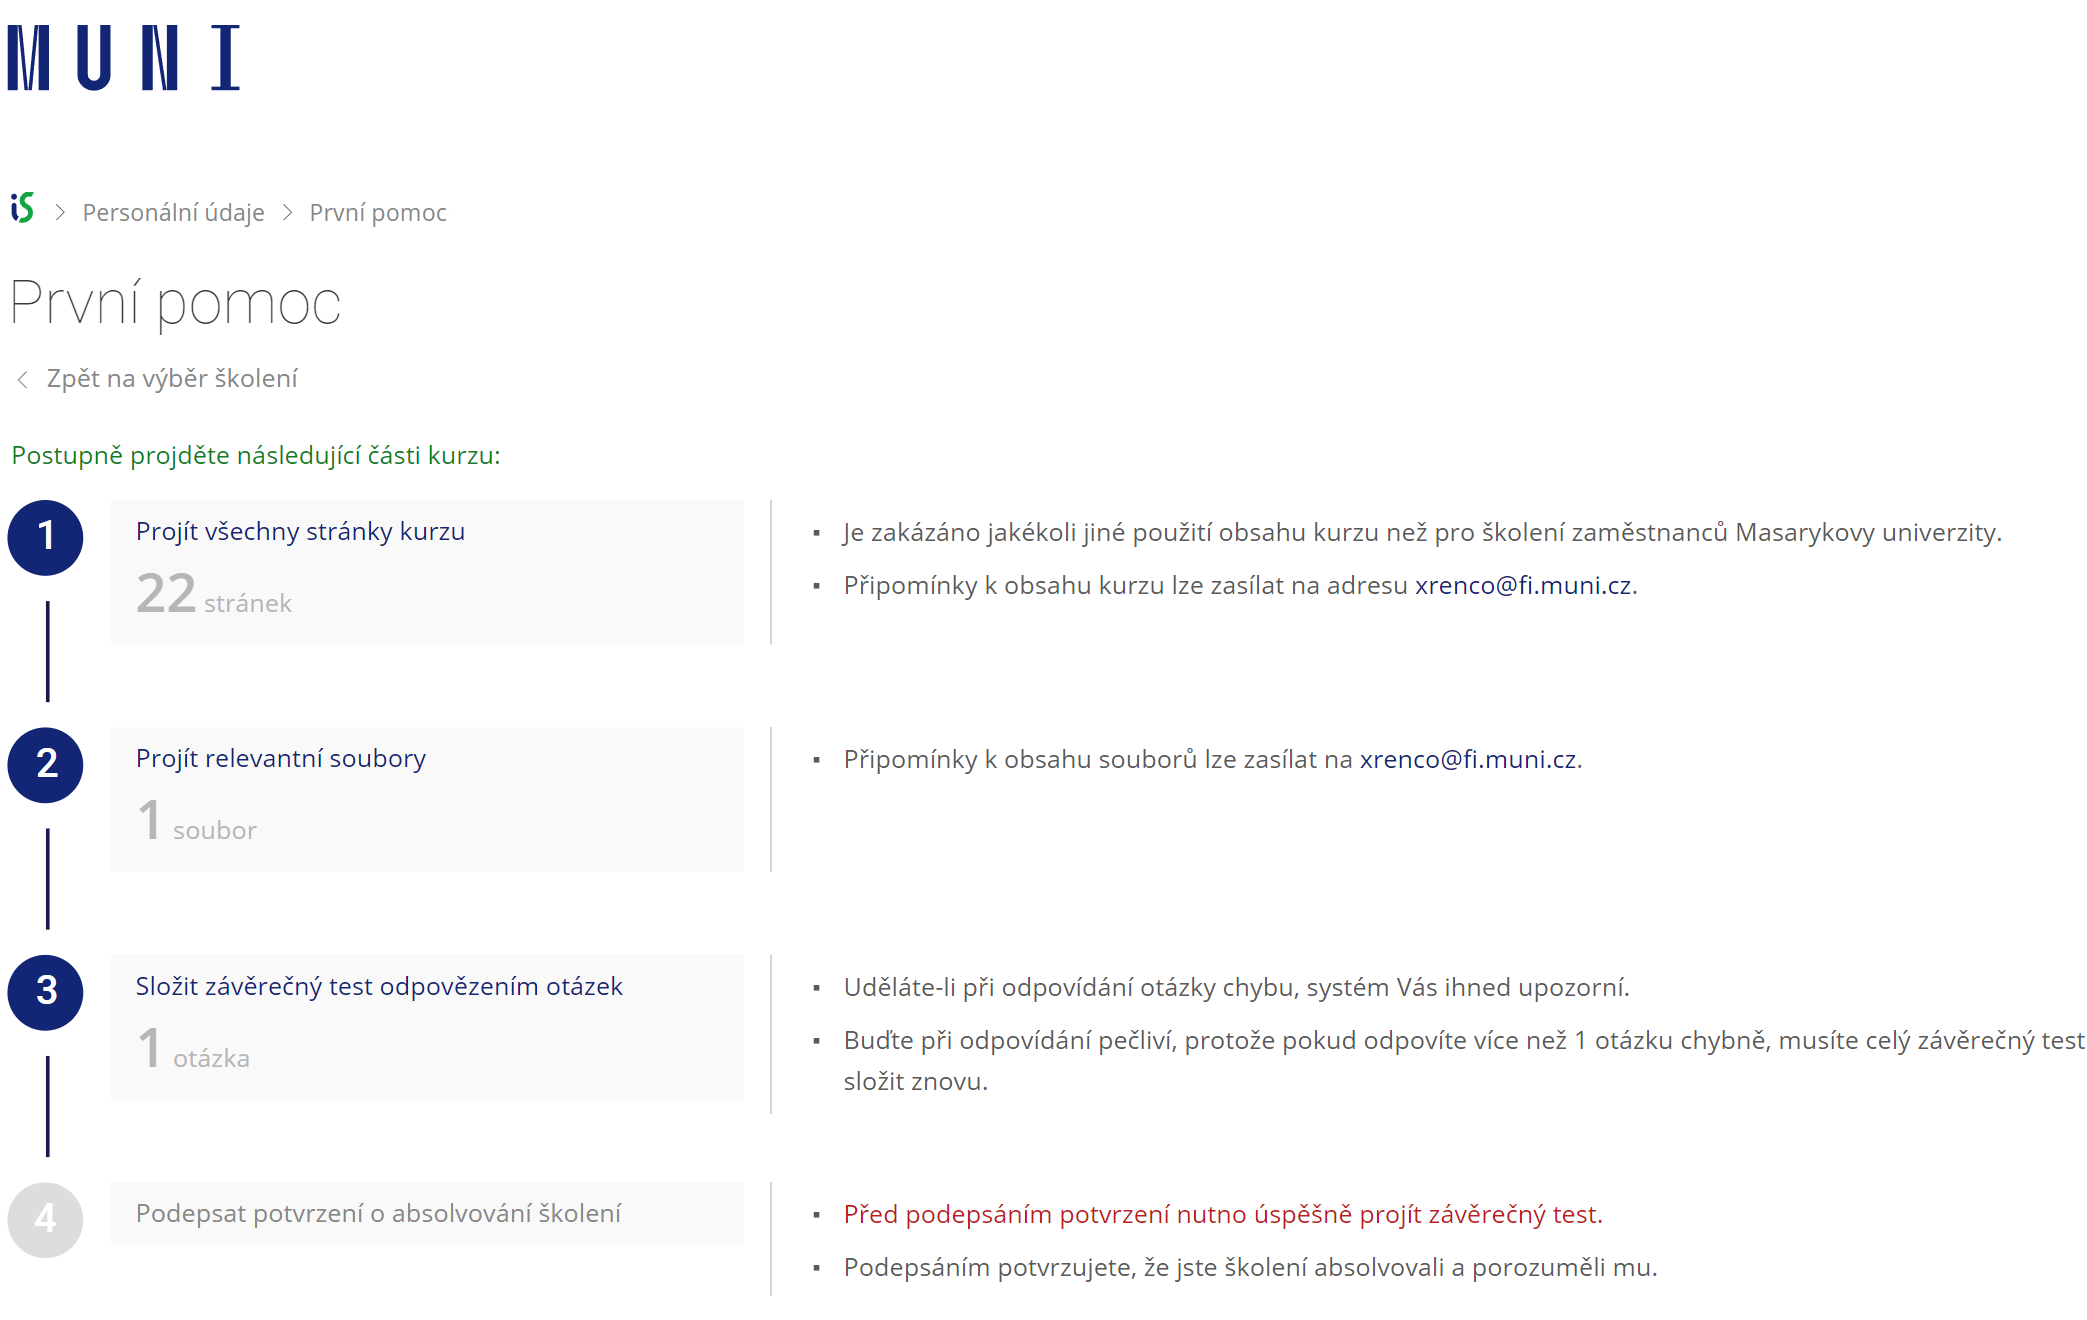
\includegraphics[width=\textwidth]{prehledvyberu.png}
  \end{center}
  \caption{Prehľad kurzu prvej pomoci v aplikácii Bozp}
  \label{obr1}
\end{figure}

\noindent
Časti sú frekventantovi sprístupňované postupne v ich číselnom poradí.
Podpísanie Potvrdenia o absolvovaní školenia je tým pádom frekventantovi umožnené až po dokončení všetkých ostatných častí kurzu.

Aplikácia Bozp poskytuje v prípade potreby možnosť prikázania školenia bez generácie dokumentácie o jeho absolvovaní. Ak sa žiadna dokumentácia negeneruje, nemôže byť od frekventanta žiadaný jej podpis. Informácia o tom, či je od frekventanta požadovaný podpis je v databáze držaná so samotným príkazom na absolvovanie školenia a nie pri špecifických školeniach a kurzoch.

Funkcia pre zobrazovanie prehľadu kurzu pred implementáciou Potvrdení zisťovala relevantné informácie iba z databázových záznamov relevantného kurzu a školenia. Pre správne vyhodnocovacie, či má medzi časti zaradiť aj podpis Potvrdenia, bolo potrebné do procesu pridať aj informácie o konkrétnom príkaze frekventanta. Podpisová časť sa tým pádom frekventantovi zobrazí iba v prípade, že to je od neho požadované z príkazu k absolvovaniu školenia.

Okrem prístupu do podpisovej časti cez prehľad obsahu kurzu je frekventantovi poskytnutý odkaz priamo na túto časť (pozri obr.~\ref{obr2}) v prípade, že splnil všetky ostatné časti kurzu. Táto úprava má za cieľ minimalizovať počet prechodov kurzami, ktoré majú dokončené ostatné časti kurzu a na absolvovanie príkazu chýba už iba podpísať Potvrdenie.

\begin{figure}
  \begin{center}
    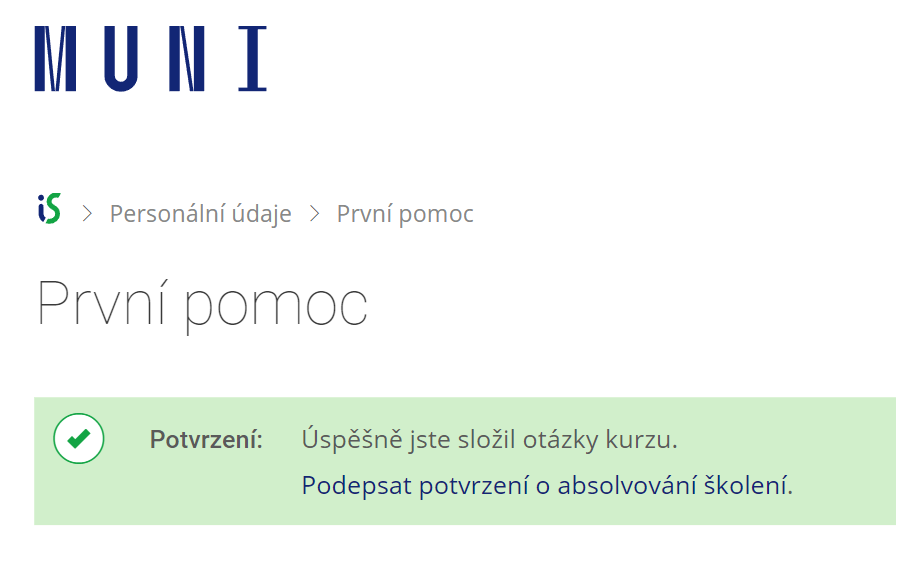
\includegraphics[width=0.8\textwidth]{odkaznapodpis.png}
  \end{center}
  \caption{Odkaz priamo na podpisovú časť kurzu}
  \label{obr2}
\end{figure}

Podľa požiadaviek rektorátu MU je príkaz k absolvovaniu školenia, u ktorého je žiadaný podpis frekventanta, považovaný za absolvovaný až po podpísaní dokumentácie o absolvovaní daného školenia. Táto požiadavka je reflektovaná do funkcií, ktoré vyhodnocujú absolvovanie príkazu, kurzu a školenia. Funkcie načítajú z databázy aj dáta, ktoré určujú, či je potrebné podpísanie dokumentácie o absolvovaní školenia, a túto podmienku zaradia medzi ostatné vyhodnocované podmienky absolvovania.

Samotná podpisová časť (pozri obr.~\ref{obr3}) vo svojom zadaní žiada frekventanta o podpis Potvrdenia. Frekventantovi zobrazí podpisované údaje, aby ich mohol skontrolovať a aby bol informovaný o obsahu dokumentu, ktorý podpisuje. Celý obsah si má frekventant možnosť stiahnuť pomocou odkazu s nápisom \enquote{Stáhnout plný obsah dokumentu}. Pod informáciami sa nachádza tlačidlo s nápisom \enquote{Podepsat}, ktoré Potvrdenie podpíše a odovzdá do spisovej služby Úradovne.

\begin{figure}
  \begin{center}
    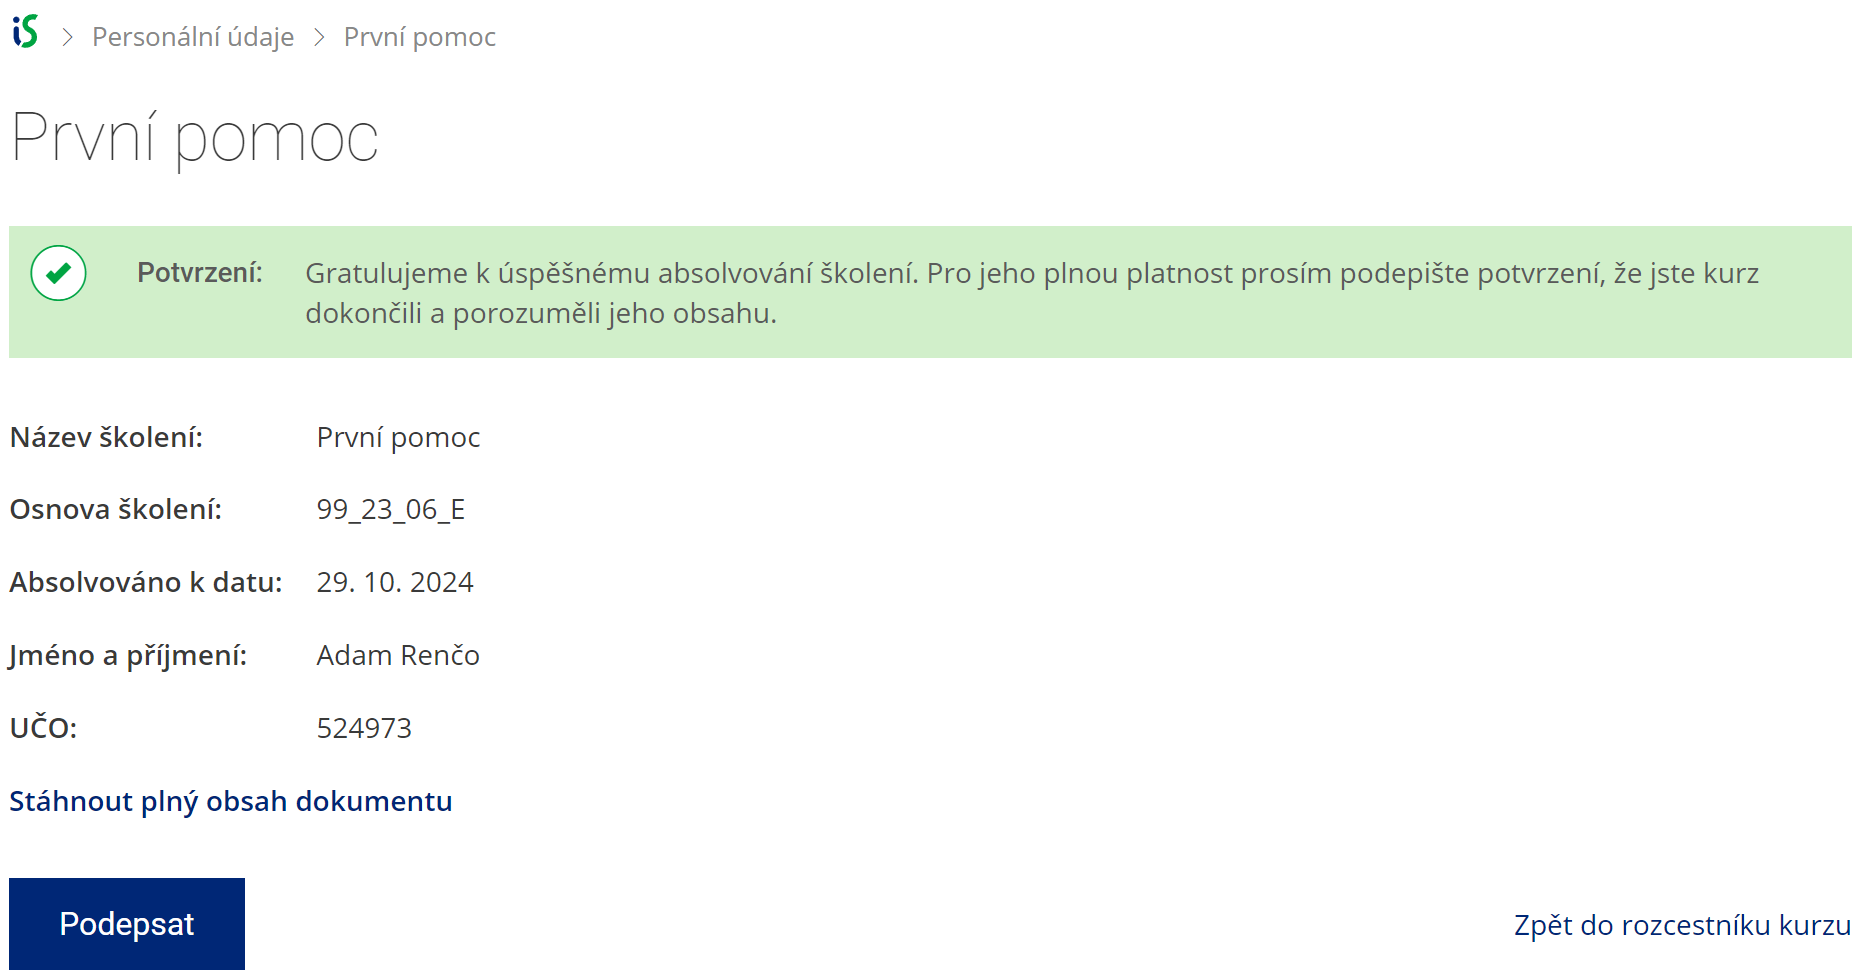
\includegraphics[width=\textwidth]{podpiscast2.png}
  \end{center}
  \caption{Podpisová časť kurzu}
  \label{obr3}
\end{figure}

\section{Prepojenie aplikácie Bozp s Úradovňou}
Potvrdenia je potrebné uchovávať v spisovej službe. Preto sú po ich podpísaní z aplikácie Bozp posielané do Úradovne. Funkcia Úradovne, ktorá vykoná tento presun, požaduje ako argumenty:

\begin{itemize}
    \item Identifikačné číslo absolventa;
    \item názov Potvrdenia;
    \item dátum absolvovania školenia;
    \item identifikačné číslo príkazu na absolvovanie školenia;
    \item Potvrdenie samotné ako dokument na uloženie do spisu; a
    \item identifikačné číslo pracoviska, ktoré bude spravovať spis Potvrdenia.
\end{itemize}
\noindent
\textbf{Identifikačné číslo absolventa:} na MU je používané univerzitné číslo osoby (UČO)\footnote{\url{https://it.muni.cz/kategorie/ucty-hesla-a-id-karty}}, ktoré ju jednoznačne identifikuje.

\noindent
\textbf{Názov Potvrdenia:} Tento názov je použitý aj ako názov spisu. Názov je tvorený spojením názvu školenia a dátumu absolvovania.

\noindent
\textbf{Dátum absolvovania školenia:} Dátum, od ktorého školenie nadobúda platnosť.

\noindent
\textbf{Identifikačné číslo príkazu na absolvovanie školenia:} Unikátny číselný kód priradený príkazu, ktorý nariaďuje absolvovanie konkrétneho školenia.

\noindent
\textbf{Potvrdenie samotné ako dokument na uloženie do spisu:} Finálne nepodpísané Potvrdenie obsahujúce relevantné informácie o absolventovi a absolvovanom školení.

\noindent
\textbf{Identifikačné číslo pracoviska:} Unikátny kód priradený pracovisku, ktoré spravuje spis Potvrdenia.

\subsection*{Kanonické pracovisko}
Pracovisko, ktoré má spravovať spis Potvrdenia nie je s príkazom ani školením priamo spojené. Preto ako identifikačné číslo pracoviska používame algoritmicky spočítané \textbf{kanonické pracovisko}.
\begin{description}
    \item[Kanonické pracovisko] je určené na základe nasledujúceho postupu:
    \begin{enumerate}
        \item \textbf{Ak má frekventant jedno alebo viac kmeňových pracovísk na MU:}
        \begin{itemize}
            \item Z týchto pracovísk sa vyberie to, ktoré má najdlhšie identifikačné číslo.
            \item Ak existuje viacero pracovísk s rovnakou dĺžkou identifikačného čísla, vyberie sa to s numericky najmenším číslom.
        \end{itemize}
        \item \textbf{Ak frekventant nemá kmeňové pracovisko na MU:}
        \begin{itemize}
            \item Postupuje sa rovnako ako v bode 1, ale výber sa uskutoční zo všetkých (aj nekmeňových) pracovísk frekventanta na MU.
        \end{itemize}
        \item \textbf{Ak frekventant nemá žiadne známe pracovisko na MU:}
        \begin{itemize}
            \item Použije sa pracovisko MU špecifikované v pravidle, podľa ktorého vznikol príkaz na absolvovanie školenia.
        \end{itemize}
        \item \textbf{Ak takéto pravidlo neexistuje:}
        \begin{itemize}
            \item Tak sa použije podľa bodov 1, 2 a 3 spočítané pracovisko osoby, ktorá príkaz založila.
        \end{itemize}
        \item \textbf{Ak osoba, ktorá príkaz založila, nie je známa alebo sa nepodarilo spočítať jej pracovisko:}
        \begin{itemize}
            \item Použije sa predvolené pracovisko Prevádzkový odbor rektorátu MU.
        \end{itemize}
    \end{enumerate}
\end{description}

\subsection*{Priloženie podpisovej doložky a zapečatenie}
Po presune výsledného Potvrdenia do Úradovne je k nemu pripojená podpisová doložka obsahujúca všetky dôležité informácie o podpísaní absolventom a následne je Potvrdenie zaradené do fronty na zapečatenie kvalifikovanou elektronickou pečaťou IS MU. Absolvent je o stave pečatenia informovaný priamo v podpisovej časti kurzu po podpísaní Potvrdenia. Zároveň je mu zobrazený odkaz na zobrazenie Potvrdenia v spise Úradovne.

Tento odkaz je generovaný Úradovňou a spolu s identifikačným číslom dokumentu je vrátený aplikácii Bozp, ktorá si ho uchováva. Odkaz sa používa na zobrazenie existujúceho Potvrdenia pri návrate absolventa k prehliadke dokončeného kurzu a podľa identifikačného čísla dokumentu sa kontroluje stav zapečatenia dokumentu v Úradovni. Aplikácia Bozp si uchováva aj presný čas vykonania podpisu pri každom prechode elektronickým kurzom, aby bolo možné presnejšie dokázať existenciu tohto úkonu.

Vzorový príklad výsledného podpísaného a zapečateného Potvrdenia sa nachádza v prílohe~\hyperref[priloha1]{1}.

\subsection*{Nasadenie Potvrdení v IS MU}
Generácia Potvrdení bola otestovaná pomocou testovacích príkladov frekventantov, školení a príkazov na ich splnenie. Následne bol podpis Potvrdení sprístupnený v relevantných kurzoch v aplikácii Bozp.

Prevádzka podpisovania Potvrdení je priebežne kontrolovaná. Databázové objekty používané v aplikácii Bozp majú nastavené prísne obmedzenia\footnote{\url{https://docs.oracle.com/cd/B13789_01/server.101/b10759/clauses002.htm}}, vďaka ktorým je možné zamedziť prípadným chybám už pred ich vznikom alebo aspoň minimalizovať spôsobené škody. Digitálne spisy obsahujúce Potvrdenia nie je potrebné kontrolovať v aplikácii Bozp, pretože sú tieto kontroly prevádzané priamo v aplikácii Úradovňa, ktorá spisy udržiava.

Potvrdenia budú naďalej zlepšované. Hlavným zameraním je úprava správcovských aplikácií, aby mali zodpovedné osoby ľahší prístup k spravovaniu tejto dokumentácie. Ďalším dôležitým rozšírením je aj pridanie možnosti zobrazenia prehľadu osôb, ktoré dokončili školenie ale nepodpísali Potvrdenie.

Úpravy sa budú týkať aj vizuálnej stránky podpisovej časti kurzov. Dizajn tejto časti bude upravený, aby bol prehľadnejší a prívetivejší.

\chapter*{Záver}
\addcontentsline{toc}{chapter}{Záver}
Cieľom tejto práce bolo previesť podpisovanie dokumentácie o absolvovaní školení a jej uchovávanie z fyzickej do digitálnej formy. Tieto zmeny vedú k zníženiu administratívnej záťaže pre absolventov aj správcov školení a zjednodušeniu celkovej prevádzky školení v IS MU.

V priebehu práce boli preskúmané dôležité právne a používateľské požiadavky týkajúce sa školení a digitálnej dokumentácie, ako aj technológie, ktoré sú pre tento účel vhodné. Na základe týchto zistení boli formulované návrhy na zlepšenie doterajšieho systému správy dokumentácie školení v IS MU. Každý z návrhov bol analyzovaný z hľadiska jeho výhod a nevýhod.

Zvoleným riešením bolo implementovať Potvrdenie o absolvovaní školenia s jednoduchým elektronickým podpisom do aplikácie Bozp v IS MU. Potvrdenia sú aplikáciou generované a možnosť ich podpisovania bola implementovaná v súlade s právnymi požiadavkami na dokumentáciu školení BOZP a PO. Proces podpisovania pomocou jednoduchého elektronického podpisu je v súlade so zákonnými nariadeniami. Fyzické Záznamy boli nahradené digitálnou dokumentáciou o absolvovaní školení, čím sa dosiahol stanovený cieľ práce.

\chapter*{Zoznam príloh}
\addcontentsline{toc}{chapter}{Zoznam príloh}

\begin{enumerate}
    \item \textbf{Príloha 1:} Vzorové potvrdenie o absolvovaní testovacieho školenia prvej pomoci.\label{priloha1}
\end{enumerate}

\printbibliography[heading=bibintoc] %% Print the bibliography.

\end{document}
